%\chapter{Introduction}

%\section{Background and Recent Research}
%\subsection{<any sub section here>}

%\subsection{Literature Survey}

%\subsubsection{<Sub-subsection title>}
%some text\cite{citation-1-name-here}, some more text

%\subsubsection{<Sub-subsection title>}
%even more text\footnote{<footnote here>}, and even more.

\section{Motivation}

This report will provide a detailed account of the processes our group
used to design and implement a database that can be used to manage
a blood donation system. Each subsection of the report will correspond to an
important feature of database design.

\section{Database Schema}
%\subsection{BDC_Employee}

\begin{tabular}{ | c | c | c | c | c | c | c | }
 \hline
 EMP_ID & BDC_ID & F_NAME & L_NAME & DESIGNATION & DAT_OF_JOIN & PASSWORD \\
 \hline
\end{tabular}

\section{Entity Relationship Diagram}
\begin{figure}[htb]
\centering
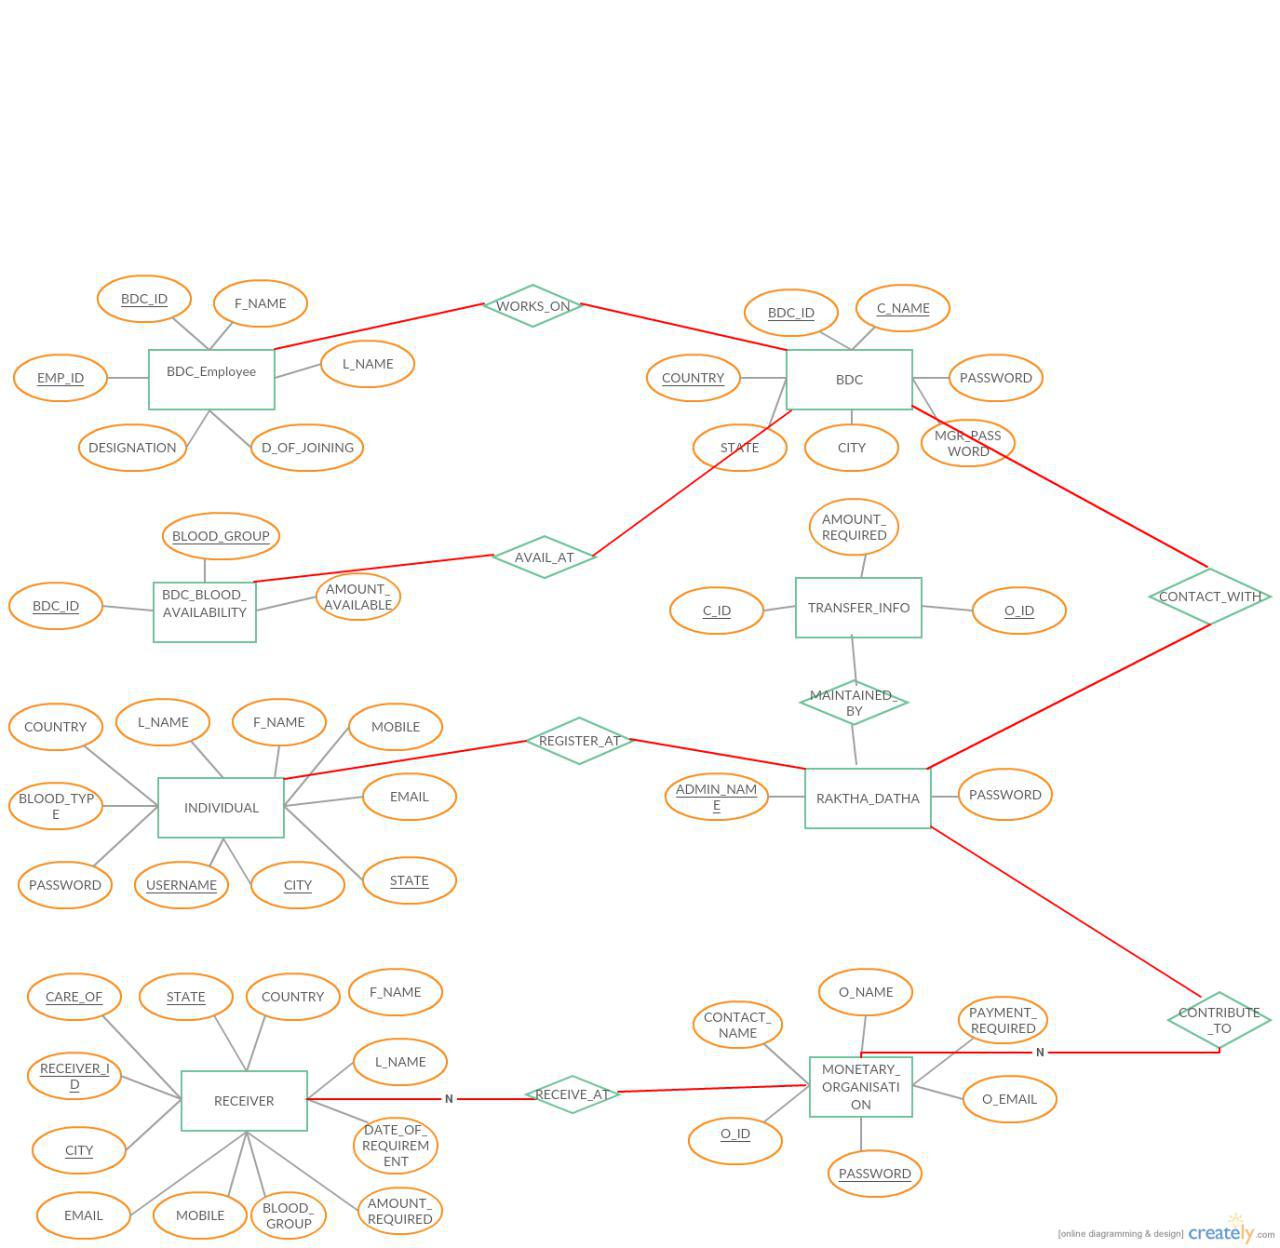
\includegraphics[scale=0.3]{./er} % e.g. insert ./image for image.png in the working directory, adjust scale as necessary
%\caption{<Caption here>}
\label{fig:label} % insert suitable label, this is used to refer to a fig from within the text as shown above
\end{figure}

\section{Glossary}
BDC_Employee : Blood Donation Centre Employee
